% Options for packages loaded elsewhere
\PassOptionsToPackage{unicode}{hyperref}
\PassOptionsToPackage{hyphens}{url}
\PassOptionsToPackage{dvipsnames,svgnames,x11names}{xcolor}
\documentclass[
  10pt,
  fontset=fandol]{ctexart}
\usepackage{xcolor}
\usepackage[margin=16mm]{geometry}
\usepackage{amsmath,amssymb}
\setcounter{secnumdepth}{-\maxdimen} % remove section numbering
\usepackage{iftex}
\ifPDFTeX
  \usepackage[T1]{fontenc}
  \usepackage[utf8]{inputenc}
  \usepackage{textcomp} % provide euro and other symbols
\else % if luatex or xetex
  \usepackage{unicode-math} % this also loads fontspec
  \defaultfontfeatures{Scale=MatchLowercase}
  \defaultfontfeatures[\rmfamily]{Ligatures=TeX,Scale=1}
\fi
\usepackage{lmodern}
\ifPDFTeX\else
  % xetex/luatex font selection
\fi
% Use upquote if available, for straight quotes in verbatim environments
\IfFileExists{upquote.sty}{\usepackage{upquote}}{}
\IfFileExists{microtype.sty}{% use microtype if available
  \usepackage[]{microtype}
  \UseMicrotypeSet[protrusion]{basicmath} % disable protrusion for tt fonts
}{}
\makeatletter
\@ifundefined{KOMAClassName}{% if non-KOMA class
  \IfFileExists{parskip.sty}{%
    \usepackage{parskip}
  }{% else
    \setlength{\parindent}{0pt}
    \setlength{\parskip}{6pt plus 2pt minus 1pt}}
}{% if KOMA class
  \KOMAoptions{parskip=half}}
\makeatother
\usepackage{graphicx}
\makeatletter
\newsavebox\pandoc@box
\newcommand*\pandocbounded[1]{% scales image to fit in text height/width
  \sbox\pandoc@box{#1}%
  \Gscale@div\@tempa{\textheight}{\dimexpr\ht\pandoc@box+\dp\pandoc@box\relax}%
  \Gscale@div\@tempb{\linewidth}{\wd\pandoc@box}%
  \ifdim\@tempb\p@<\@tempa\p@\let\@tempa\@tempb\fi% select the smaller of both
  \ifdim\@tempa\p@<\p@\scalebox{\@tempa}{\usebox\pandoc@box}%
  \else\usebox{\pandoc@box}%
  \fi%
}
% Set default figure placement to htbp
\def\fps@figure{htbp}
\makeatother
\setlength{\emergencystretch}{3em} % prevent overfull lines
\providecommand{\tightlist}{%
  \setlength{\itemsep}{0pt}\setlength{\parskip}{0pt}}
\usepackage{amsmath,amssymb,mathtools,needspace}
\xeCJKDeclareCharClass{CJK}{"2032,"0400->"04FF,"2160->"216B,"2460->"2473,"25A0,"25C7,"25CB,"25CF}
\IfFontExistsTF{Arial Unicode MS}{\xeCJKsetup{AutoFallBack=true}\setCJKfallbackfamilyfont{\CJKrmdefault}{Arial Unicode MS}}{}
\setcounter{secnumdepth}{0}
\setlength{\emergencystretch}{2em}
\allowdisplaybreaks
\usepackage{bookmark}
\IfFileExists{xurl.sty}{\usepackage{xurl}}{} % add URL line breaks if available
\urlstyle{same}
\hypersetup{
  pdftitle={Householder 方法},
  colorlinks=true,
  linkcolor={Maroon},
  filecolor={Maroon},
  citecolor={Blue},
  urlcolor={Blue},
  pdfcreator={LaTeX via pandoc}}

\title{Householder 方法}
\author{}
\date{}

\begin{document}
\maketitle

\subsection{9.3 Householder 方法}\label{householder-ux65b9ux6cd5}

\subsubsection{9.3.1 引言}\label{ux5f15ux8a00}

前面几节讨论的是求解矩阵最大（小）特征值及其对应特征向量的方法。若要求求出所有特征值及其特征向量，应该用什么方法呢？下面将讨论的以正交相似变换为基础的一类方法即是解决这类问题的方法。

首先，讨论对于一般实矩阵 \(A\in\mathbf R^{n\times n}\) 利用正交相似变换约化到什么程度的问题。由代数知识可知如下定理。

\textbf{定理 9.10} 设 \(A\in\mathbf R^{n\times n}\)，则存在一个正交阵 \(R\)，使

\[
R^{\mathrm T}AR=\begin{pmatrix}
T_{11}&T_{12}&\cdots&T_{1s}\\
&T_{22}&\cdots&T_{2s}\\
&&\ddots&\vdots\\
&&&T_{ss}
\end{pmatrix},
\]

其中对角块为一阶或二阶矩阵，每一个一阶对角块即为 \(A\) 的实特征值，每一个二阶对角块的两个特征值是 \(A\) 的一对共轭复特征值。

\textbf{定义 9.2} 一方阵 \(B\)，如果当 \(i>j+1\) 时有 \(b_{ij}=0\)，则称 \(B\) 为上 Hessenberg 阵，即

\[
B=\begin{pmatrix}
b_{11}&b_{12}&\cdots&b_{1n}\\
b_{21}&b_{22}&\cdots&b_{2n}\\
&\ddots&\ddots&\vdots\\
&&b_{n,n-1}&b_{nn}
\end{pmatrix}.
\]

本节讨论如下两个问题：

（1）用正交相似变换约化一般实矩阵为上 Hessenberg 阵；

（2）用正交相似变换约化对称阵为三对角阵。

这样，求原矩阵特征值问题，就转化为求上 Hessenberg 阵或对称三对角阵的特征值问题。

\textbf{定义 9.3} 设向量 \(w\) 满足 \(\|w\|_2=1\)，矩阵 \(H=I-2ww^{\mathrm T}\) 称为初等反射阵，记作 \(H(w)\)，即

\[
H(w)=\begin{pmatrix}
1-2w_1^2&-2w_1w_2&\cdots&-2w_1w_n\\
-2w_2w_1&1-2w_2^2&\ddots&\vdots\\
\vdots&\ddots&\ddots&-2w_{n-1}w_n\\
-2w_nw_1&\cdots&-2w_nw_{n-1}&1-2w_n^2
\end{pmatrix},
\]

\href{../../source-images/pdf-244.jpeg}{原页图像}

其中

\[
w=(w_1,w_2,\cdots,w_n)^{\mathrm T}.
\]

\textbf{定理 9.11} 初等反射阵 \(H\) 是对称阵（\(H^{\mathrm T}=H\)）、正交阵（\(H^{\mathrm T}H=I\)）和对合阵（\(H^2=I\)）。

\textbf{证明} 只证 \(H\) 的正交性，其他显然。

\[
H^{\mathrm T}H=H^2=(I-2ww^{\mathrm T})(I-2ww^{\mathrm T})=I-4ww^{\mathrm T}+4w(w^{\mathrm T}w)w^{\mathrm T}=I.
\]

设向量 \(u\ne0\)，则显然 \(H=I-2\dfrac{uu^{\mathrm T}}{\|u\|_2^2}\) 是一个初等反射阵。

下面考察初等反射阵的几何意义。考虑以 \(w\) 为法向量过原点 \(O\) 的超平面

\[
S:w^{\mathrm T}x=0.
\]

设任意向量 \(v\in\mathbf R^n\)，则 \(v=x+y\)，其中 \(x\in S,y\in S^{\perp}\)。于是

\[
Hx=(I-2ww^{\mathrm T})x=x-2ww^{\mathrm T}x=x.
\]

对于 \(y\in S^{\perp}\)，易知 \(Hy=-y\)，从而对于任意向量 \(v\in\mathbf R^n\)，总有

\[
Hv=x-y=v',
\]

其中 \(v'\) 为 \(v\) 关于平面 \(S\) 的镜面反射（见图 9.1）。

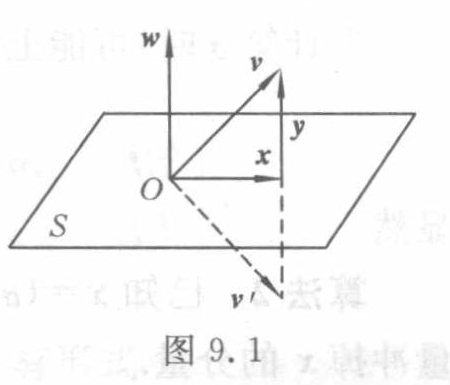
\includegraphics[width=0.85\linewidth,height=\textheight,keepaspectratio,alt={图 9.1，初等反射阵的几何意义，原图裁切}]{../assets/ch09a/fig-9-1.png}

图 9.1（原图裁切）。图中符号为 \(w,\allowbreak v,\allowbreak x,\allowbreak y,\allowbreak O,\allowbreak S,\allowbreak v'\)。超平面 \(S\) 经过原点 \(O\)，\(w\) 为法向量；\(v=x+y\) 分解为平面内分量 \(x\) 与垂直分量 \(y\)，\(v'\) 位于平面另一侧，表示镜面反射所得 \(x-y\)。原图用虚线连接 \(O\)、\(v'\) 端点及垂直分量方向。

初等反射阵在计算上的意义是它能用来约化矩阵，例如设向量 \(a\ne0\)，可选择一初等反射阵 \(H\) 使 \(H_a=\sigma e_1\)。这种约化矩阵的方法称为 Householder 方法。为此给出下面定理。

\textbf{定理 9.12} 设 \(x,y\) 为两个不相等的 \(n\) 维向量，\(\|x\|_2=\|y\|_2\)，则存在一个初等反射阵 \(H\)，使 \(Hx=y\)。

\textbf{证明} 令 \(w=\dfrac{x-y}{\|x-y\|_2}\)，则得到一个初等反射阵

\[
H=I-2ww^{\mathrm T}=I-2\frac{(x-y)}{\|x-y\|_2^2}(x^{\mathrm T}-y^{\mathrm T}),
\]

而且

\[
Hx=x-2\frac{x-y}{\|x-y\|_2^2}(x^{\mathrm T}-y^{\mathrm T})x=x-2\frac{(x-y)(x^{\mathrm T}x-y^{\mathrm T}x)}{\|x-y\|_2^2},
\]

因为

\[
\|x-y\|_2^2=(x-y)^{\mathrm T}(x-y)=2(x^{\mathrm T}x-y^{\mathrm T}x),
\]

所以

\[
Hx=x-(x-y)=y.
\]

易知，\(w=\dfrac{x-y}{\|x-y\|_2}\) 是使 \(Hx=y\) 成立的唯一长度等于 1 的向量（不计符号）。

\textbf{推论} 设向量 \(x\in\mathbf R^n\ (x\ne0)\)，\(\sigma=\pm\|x\|_2\)，且 \(x\ne-\sigma e_1\)，则存在一个初等反射阵

\[
H=I-2\frac{uu^{\mathrm T}}{\|u\|_2^2}\equiv I-\rho^{-1}uu^{\mathrm T},
\]

使 \(Hx=-\sigma e_1\)，其中 \(u=x+\sigma e_1\)，\(\rho=\|u\|_2^2/2\)。

设

\[
x=(\alpha_1,\alpha_2,\cdots,\alpha_n)^{\mathrm T}\ne0,\quad u=(u_1,u_2,\cdots,u_n)^{\mathrm T},
\]

\begin{quote}
\textbf{校注（agent 补充，ch09a-E008）} 在``可选择一初等反射阵 \(H\) 使''后，原图把 \(a\) 印在 \(H\) 的下标位置，故照录为 \(H_a=\sigma e_1\)。依本段语义及随后定理的矩阵作用，应为乘积 \(Ha=\sigma e_1\)；疑为原书排版错误。见\href{../assets/ch09a/review-p244-Ha.png}{放大原式}。
\end{quote}

\href{../../source-images/pdf-245.jpeg}{原页图像}

则

\[
u=(\alpha_1+\sigma,\alpha_2,\cdots,\alpha_n)^{\mathrm T},
\]

\[
\rho=\frac12\|u\|_2^2=\frac12\left[(\alpha_1+\sigma)^2+\alpha_2^2+\cdots+\alpha_n^2\right]=\sigma(\sigma+\alpha_1).
\]

如果 \(\sigma\) 和 \(\alpha_1\) 异号，那么计算 \(\alpha_1+\sigma\) 时有效数字可能损失，取 \(\sigma\) 和 \(\alpha_1\) 有相同的符号，即取

\[
\sigma=\operatorname{sgn}(\alpha_1)\|x\|_2.
\]

\textbf{算法 1} 已知向量 \(x=(\alpha_1,\alpha_2,\cdots,\alpha_n)^{\mathrm T}\ne0\)，本算法算出 \(\sigma,\rho\) 及 \(u\)，使 \((I-\rho^{-1}uu^{\mathrm T})x=-\sigma e_1\)，\(u\) 的分量冲掉 \(x\) 的分量。

\textbf{步 1} 计算 \(\sigma=\operatorname{sgn}(\alpha_1)\left(\displaystyle\sum_{i=1}^n\alpha_i^2\right)^{\frac12}\)。

\textbf{步 2} \(\alpha_1\to u_1=\alpha_1+\sigma\)。

\textbf{步 3} \(\rho=\sigma u_1\)。

在计算 \(\sigma\) 时，可能上溢或下溢。为了避免溢出，将 \(x\) 规范化

\[
\eta=\max_i|\alpha_i|,\quad x'=\frac{x}{\eta},
\]

显然

\[
\sigma'=\sigma/\eta,\quad H'=H.
\]

\textbf{算法 2} 已知 \(x=(\alpha_1,\alpha_2,\cdots,\alpha_n)^{\mathrm T}\ne0\)，本算法算出 \(H\) 及 \(\sigma\) 使 \(Hx=-\sigma e_1\)，\(u\) 的分量冲掉 \(x\) 的分量。

\textbf{步 1} \(\eta=\max_i|\alpha_i|\)。

\textbf{步 2} \(\alpha_i\leftarrow u_i=\dfrac{\alpha_i}{\eta}\quad(i=1,2,\cdots,n)\)。

\textbf{步 3} \(\sigma=\operatorname{sgn}(u_1)\left(\displaystyle\sum_{i=1}^nu_i^2\right)^{\frac12}\)。

\textbf{步 4} \(u_1\leftarrow u_1+\sigma\)。

\textbf{步 5} \(\rho=\sigma u_1\)。

\textbf{步 6} \(\sigma\leftarrow\eta\sigma\)。

关于 \(HA\) 的计算，设 \(A=(a_1,a_2,\cdots,a_n)\)，其中 \(a_i\) 为 \(A\) 的第 \(i\) 列向量，则

\[
HA=(Ha_1,Ha_2,\cdots,Ha_n),
\]

因此计算 \(HA\) 就是要计算

\[
Ha_i=(I-\rho^{-1}uu^{\mathrm T})a_i=a_i-(\rho^{-1}u^{\mathrm T}a_i)u\quad(i=1,2,\cdots,n).
\]

于是计算 \(Ha_i\) 只需要计算两向量的数量积和两向量的加法即可，且计算 \(HA\) 共需要 \(2n^2\) 次乘法运算。

\subsubsection{9.3.2 用正交相似变换约化矩阵}\label{ux7528ux6b63ux4ea4ux76f8ux4f3cux53d8ux6362ux7ea6ux5316ux77e9ux9635}

下面考虑用初等反射阵来正交相似约化一般矩阵和对称矩阵。设

\href{../../source-images/pdf-246.jpeg}{原页图像}

\[
A=\left(\begin{array}{c|ccc}
a_{11}&a_{12}&\cdots&a_{1n}\\\hline
a_{21}&a_{22}&\cdots&a_{2n}\\
\vdots&\vdots&&\vdots\\
a_{n1}&a_{n2}&\cdots&a_{nn}
\end{array}\right)
\equiv\begin{pmatrix}
a_{11}&A_{12}^{(1)}\\
a_{21}^{(1)}&A_{22}^{(1)}
\end{pmatrix},
\]

\textbf{步 1} 不妨设 \(a_{21}^{(1)}\ne0\)，否则这一步不需约化，选择初等反射阵 \(R_1\) 使 \(R_1a_{21}^{(1)}=-\sigma_1e_1\)，其中

\[
\left\{
\begin{aligned}
\sigma_1&=\operatorname{sgn}(a_{21})\left(\sum_{i=2}^na_{i1}^2\right)^{\frac12},\\
u_1&=a_{21}^{(1)}+\sigma_1e_1,\\
\rho_1&=\frac12\|u_1\|_2^2=\sigma_1(\sigma_1+a_{21}),\\
R_1&=I-\rho_1^{-1}u_1u_1^{\mathrm T}.
\end{aligned}
\right.
\tag{9.3.1}
\]

令 \(U_1=\begin{pmatrix}I&0\\0&R_1\end{pmatrix}\)，则

\[
A_2=U_1A_1U_1=\begin{pmatrix}
a_{11}&A_{21}^{(1)}R_1\\
R_1a_{21}^{(1)}&R_1A_{22}^{(1)}R_1
\end{pmatrix}
\equiv\begin{pmatrix}
A_{11}^{(2)}&a_{12}^{(2)}&A_{13}^{(2)}\\
O&a_{22}^{(2)}&A_{23}^{(2)}
\end{pmatrix},
\]

其中 \(A_{11}^{(2)}\in\mathbf R^{2\times1},\allowbreak \quad a_{22}^{(2)}\in\mathbf R^{n-2},\allowbreak \quad A_{23}^{(2)}\in\mathbf R^{(n-2)\times(n-2)}\)。

\textbf{步 \(k\)} 设对 \(A\) 已进行了第 \(k-1\) 步正交相似约化，即 \(A_k\) 有形式

\[
\begin{aligned}
A_k&=U_{k-1}A_{k-1}U_{k-1}\\
&=\left(\begin{array}{ccc|c|ccc}
a_{11}&a_{12}^{(2)}&\cdots&a_{1k}^{(k)}&a_{1,k+1}^{(k)}&\cdots&a_{1n}^{(k)}\\
-\sigma_1&a_{22}^{(2)}&\cdots&a_{2k}^{(k)}&a_{2,k+1}^{(k)}&\cdots&a_{2n}^{(k)}\\
&\ddots&\ddots&\vdots&\vdots&&\vdots\\
&&-\sigma_{k-1}&a_{kk}^{(k)}&a_{k,k+1}^{(k)}&\cdots&a_{k,n}^{(k)}\\\hline
&&&a_{k+1,k}^{(k)}&a_{k+1,k+1}^{(k)}&\cdots&a_{k+1,n}^{(k)}\\
&&&\vdots&\vdots&&\vdots\\
&&&a_{nk}^{(k)}&a_{n,k+1}^{(k)}&\cdots&a_{nn}^{(k)}
\end{array}\right)\\
&\equiv\begin{pmatrix}
A_{11}^{(k)}&a_{12}^{(k)}&A_{13}^{(k)}\\
O&a_{22}^{(k)}&A_{23}^{(k)}
\end{pmatrix},
\end{aligned}
\]

其中 \(A_{11}^{(k)}\in\mathbf R^{k\times(k-1)},\allowbreak \quad a_{22}^{(k)}\in\mathbf R^{n-k},\allowbreak \quad A_{23}^{(k)}\in\mathbf R^{(n-k)\times(n-k)}\)。

设 \(a_{22}^{(k)}\ne0\)，选择初等反射阵 \(R_k\)，使 \(R_ka_{22}^{(k)}=-\sigma_ke_1\)，其中

\[
\left\{
\begin{aligned}
\sigma_k&=\operatorname{sgn}(a_{k+1,k}^{(k)})\left(\sum_{i=k+1}^na_{ik}^2\right)^{\frac12},\\
u_k&=a_{22}^{(k)}+\sigma_ke_1,\\
\rho_k&=\frac12\|u_k\|_2^2=\sigma_k(\sigma_k+a_{k+1,n}^{(k)}),\\
R_k&=I-\rho_k^{-1}u_ku_k^{\mathrm T}.
\end{aligned}
\right.
\tag{9.3.2}
\]

\begin{quote}
\textbf{校注（agent 补充，ch09a-E009）} 本页 \(A_2\) 的二阶分块表达式右上块原印 \(A_{21}^{(1)}R_1\)，已照录。由页首定义的右上块 \(A_{12}^{(1)}\) 和 \(U_1\) 的分块乘法，此处应为 \(A_{12}^{(1)}R_1\)。见\href{../assets/ch09a/review-p246-initial-partition.png}{页首分块}和\href{../assets/ch09a/review-p246-A-2.png}{放大原式}。

\textbf{校注（agent 补充，ch09a-E010）} 式（9.3.2）原图 \(\sigma_k\) 求和内为 \(a_{ik}^2\)，未印迭代上标；\(\rho_k\) 最后一个矩阵元为 \(a_{k+1,n}^{(k)}\)，均照录。由本页 \(a_{22}^{(k)}=(a_{k+1,k}^{(k)},\ldots,a_{nk}^{(k)})^{\mathrm T}\) 和 \(u_k=a_{22}^{(k)}+\sigma_ke_1\)，求和应使用当前列元素 \((a_{ik}^{(k)})^2\)，而范数平方恒等式给出 \(\rho_k=\sigma_k(\sigma_k+a_{k+1,k}^{(k)})\)。故前者疑漏迭代上标，后者列下标疑将 \(k\) 印成 \(n\)。见\href{../assets/ch09a/review-p246-9-3-2.png}{放大原式}。
\end{quote}

\href{../../source-images/pdf-247.jpeg}{原页}

设 \(U_k=\begin{pmatrix}I&O\\O&R_k\end{pmatrix}\)，则

\[
A_{k+1}=U_kA_kU_k=
\begin{pmatrix}
A_{11}^{(k)}&a_{12}^{(k)}&A_{13}^{(k)}R_k\\
O&R_ka_{22}^{(k)}&R_kA_{23}^{(k)}R_k
\end{pmatrix}
=
\begin{pmatrix}
A_{11}^{(k)}&a_{12}^{(k)}&A_{13}^{(k)}R_k\\
O&-\sigma_ke_1&R_kA_{23}^{(k)}R_k
\end{pmatrix}.
\tag{9.3.3}
\]

由式（9.3.3）知，\(A_{k+1}\) 的左上角 \(k+1\) 阶子阵为上 Hessenberg 阵，从而约化又进了一步，重复这过程，直到

\[
U_{n-2}\cdots U_2U_1AU_1U_2\cdots U_{n-2}
=\begin{pmatrix}
a_{11}&\times&\times&\cdots&\times\\
-\sigma_1&a_{22}^{(2)}&\times&\cdots&\times\\
&-\sigma_2&a_{33}^{(3)}&\ddots&\vdots\\
&&\ddots&\ddots&\times\\
&&&-\sigma_{n-1}&a_{nn}^{(n-1)}
\end{pmatrix}=A_{n-1}.
\]

总结上述讨论，有如下定理。

\textbf{定理 9.13}　如果 \(A\in\mathbb R^{n\times n}\)，则存在初等反射阵 \(U_1,U_2,\cdots,U_{n-2}\)，使

\[
U_{n-2}\cdots U_2U_1AU_1U_2\cdots U_{n-2}=C\quad\text{（上 Hessenberg 阵）}.
\]

在 \(A_k\to A_{k+1}=U_kA_kU_k\) 的进一步约化中，需要计算 \(R_k\) 和 \(A_{13}^{(k)}R_k\)，\(R_kA_{23}^{(k)}R_k\)。用初等反射阵正交相似约化 \(A\) 为上 Hessenberg 阵，大约需要 \(\dfrac53n^3\) 次乘法运算。

由于 \(U_k\) 都是正交阵，所以 \(A_1\sim A_2\sim\cdots\sim A_{n-1}\)。求 \(A\) 的特征值问题，就转化为求上 Hessenberg 阵 \(C\) 的特征值问题。由定理 9.13，记 \(P=U_{n-2}\cdots U_2U_1\)，则

\[
PAP^{\mathrm T}=C.
\]

设 \(y\) 是 \(C\) 的对应特征值 \(\lambda\) 的特征向量，则 \(P^{\mathrm T}y\) 为 \(A\) 的对应特征值 \(\lambda\) 的特征向量，且

\[
P^{\mathrm T}y=U_1U_2\cdots U_{n-2}y
=(I-\lambda_1^{-1}u_1u_1^{\mathrm T})\cdots(I-\lambda_{n-2}^{-1}u_{n-2}u_{n-2}^{\mathrm T})y.
\]

\textbf{定理 9.14}　如果 \(A\in\mathbb R^{n\times n}\) 为对称阵，则存在初等反射阵 \(U_1,U_2,\cdots,U_{n-2}\)，使

\[
U_{n-2}\cdots U_2U_1AU_1U_2\cdots U_{n-2}=A_{n-1}
=\begin{pmatrix}
c_1&b_1&&&\\
b_1&c_2&b_2&&\\
&\ddots&\ddots&\ddots&\\
&&b_{n-2}&c_{n-1}&b_{n-1}\\
&&&b_{n-1}&c_n
\end{pmatrix}\equiv C.
\]

\textbf{证明}　由定理 9.13，存在初等反射阵 \(U_1,U_2,\cdots,U_{n-2}\)，使 \(A_{n-1}\) 为上 Hessenberg 阵，但 \(A_{n-1}\) 又为对称阵，因此 \(A_{n-1}\) 为对称三对角阵。

由上面讨论可知，在由 \(A_k\to A_{k+1}=U_kA_kU_k\) 一步计算过程中，只需计算 \(R_k\) 和 \(R_kA_{23}^{(k)}R_k\)。由于 \(A\) 的对称性，故只需计算 \(R_kA_{23}^{(k)}R_k\) 的对角线下面的元素。注意到

\[
R_kA_{23}^{(k)}R_k=(I-\rho_k^{-1}u_ku_k^{\mathrm T})(A_{23}^{(k)}-\rho_k^{-1}A_{23}^{(k)}u_ku_k^{\mathrm T}),
\]

\begin{quote}
校注（agent 补充）：本页 \(P^{\mathrm T}y\) 展开式原印为 \(\lambda_1^{-1}\)、\(\lambda_{n-2}^{-1}\)，而同页下方及次页初等反射阵的归一化因子使用 \(\rho_k^{-1}\)。此处保留原印 \(\lambda\)，记为疑似原书符号不一致。
\end{quote}

\href{../../source-images/pdf-248.jpeg}{原页}

引进记号

\[
r_k=\rho_k^{-1}A_{23}^{(k)}u_k,\qquad
 t_k=r_k-\frac{\rho_k^{-1}}2(u_k^{\mathrm T}r_k)u_k,
\]

则

\[
R_kA_{23}^{(k)}R_k=A_{23}^{(k)}-u_kt_k^{\mathrm T}-t_ku_k^{\mathrm T}
\quad(i=k+1,\cdots,n;\ j=k+1,\cdots,i).
\]

\textbf{算法 3}　正交相似约化对称阵为对称三对角阵。设 \(A\in\mathbb R^{n\times n}\) 是对称阵，本算法确定初等反射阵 \(U_1,U_2,\cdots,U_{n-2}\)，使 \(U_{n-2}\cdots U_1AU_1\cdots U_{n-2}=C\)（对称三对角阵），\(C\) 的对角元 \(c_i\) 存放在单元 \(c_1,c_2,\cdots,c_n\) 中，\(C\) 的非对角元 \(b_i\) 存放在单元 \(b_1,b_2,\cdots,b_{n-1}\) 中。单元 \(b_1,b_2,\cdots,b_n\) 最初可用来存放 \(r_k\) 及 \(t_k\) 的分量，确定 \(U_k\) 的向量 \(u_k\) 的分量 \(u_{k+1,k},\cdots,u_{nk}\)，存放在 \(A\) 的相应位置。\(\rho_k\) 冲掉 \(a_{kk}\)。约化 \(A\) 的结果冲掉 \(A\)，数组 \(A\) 的上部元素不变。如果步 \(k\) 不需要变换，则置 \(\rho_k\) 为零。

对于 \(k=1,2,\cdots,n-2\)，做到 \(L\)。

\textbf{步 1}　\(c_k=a_{kk}\)。

\textbf{步 2}　确定变换：

（1）计算 \(\eta=\max\limits_{k+1\leq i\leq n}|a_{ik}|\)；

（2）如果 \(\eta=0\)，则

\[
\begin{cases}
a_{kk}\to\rho_k=0,\\
b_k\to0,\\
\text{转 }L,\text{否则继续};
\end{cases}
\]

（3）计算 \(a_{ik}\leftarrow u_{ik}=a_{ik}/\eta\quad(i=k+1,\cdots,n)\)；

（4）\(\sigma=\operatorname{sgn}(u_{k+1,k})\sqrt{u_{k+1,k}^2+\cdots+u_{nk}^2}\)；

（5）\(u_{k+1,k}\leftarrow u_{k+1,k}+\sigma\)；

（6）\(a_{kk}\leftarrow\rho_k=\sigma u_{k+1,k}\)；

（7）\(b_k\leftarrow-\sigma\eta\)。

\textbf{步 3}　应用变换：

（1）\(\sigma=0\)；

（2）计算 \(A_{23}^{(k)}u_k\) 及 \(u_k^{\mathrm T}r_k\)，对于 \(i=k+1,\cdots,n\)，做

\[
\begin{cases}
b_i\leftarrow s=\displaystyle\sum_{j=k+1}^{n}a_{ij}u_{jk}+\displaystyle\sum_{j=i+1}^{n}a_{ji}u_{jk},\\
\sigma\leftarrow\sigma+su_{ik};
\end{cases}
\]

（3）计算 \(t_k\)

\[
b_i\leftarrow\rho_k^{-1}\left(b_i-\rho_k^{-1}\frac\sigma2u_{ik}\right)
\quad(i=k+1,\cdots,n);
\]

（4）计算 \(R_kA_{23}^{(k)}R_k\)

对于 \(i=k+1,\allowbreak k+2,\allowbreak \cdots,\allowbreak n;\ j=k+1,\allowbreak \cdots,\allowbreak i\)，做 \(a_{ij}\leftarrow a_{ij}-u_{ik}b_j-b_iu_{jk}\)。

\(L\)：继续循环。

对于 \(k=n-1\)，有

\[
c_{n-1}\leftarrow a_{n-1,n-1},\qquad c_n\leftarrow a_{nn},\qquad b_{n-1}\leftarrow a_{n,n-1}.
\]

\begin{quote}
校注（agent 补充）：算法 3 步 3（2）第一个求和上限原印为 \(n\)。按只存储、更新下三角部分的算法结构，该上限疑应为 \(i\)，否则 \(j>i\) 的项与第二个求和重叠，且会读入未更新的上三角元素。正文保留原印，列为疑似原书错误。
\end{quote}

\href{../../source-images/pdf-249.jpeg}{原页}

将对称阵 \(A\) 用初等反射阵正交相似约化为对称三对角阵约需做 \(\dfrac23n^3\) 次乘法运算。

用正交矩阵进行约化，有一些特点，如构造的 \(U_k\) 容易求逆，且 \(U_k\) 的元素数量级不大，因此这个算法是十分稳定的。

\textbf{例 9.5}　用 Householder 方法将下述矩阵化为上 Hessenberg 阵

\[
A_1=A=\begin{pmatrix}-4&-3&-7\\2&3&2\\4&2&7\end{pmatrix}.
\]

\textbf{解}　（1）对于 \(k=1\)，确定变换 \(U_1=\begin{pmatrix}1&\begin{matrix}0&0\end{matrix}\\\begin{matrix}0\\0\end{matrix}&R_1\end{pmatrix}\)，\(a_{21}^{(1)}=\begin{pmatrix}2\\4\end{pmatrix}\)，其中 \(R_1\) 为初等反射阵且使

\[
R_1a_{21}^{(1)}=-\sigma_1\begin{pmatrix}1\\0\end{pmatrix},\qquad
\sigma_1=\|a_{21}^{(1)}\|_2=\sqrt{20}\approx4.472\,136,
\]

\[
u_1=a_{21}^{(1)}+\sigma_1\rho_1=\begin{pmatrix}2+\sqrt{20}\\4\end{pmatrix}
\approx\begin{pmatrix}6.472\,136\\4\end{pmatrix},
\]

\[
\rho_1=\sigma_1(\sigma_1+a_{21})=\sqrt{20}(\sqrt{20}+2)\approx28.944\,27,\qquad
R_1=I-\rho_1^{-1}u_1u_1^{\mathrm T}.
\]

（2）计算 \(R_1A_{22}^{(1)}\)。记

\[
A_{22}^{(1)}=\begin{pmatrix}3&2\\2&7\end{pmatrix}\equiv(a_1,a_2),
\]

于是

\[
R_1A_{22}^{(1)}=(R_1a_1,R_1a_2)
=\begin{pmatrix}-3.130\,496&-7.155\,419\\-1.788\,855&1.341\,640\end{pmatrix},
\]

其中

\[
R_1a_i=(I-\rho_1^{-1}u_1u_1^{\mathrm T})a_i
=a_i-(\rho_1^{-1}u_1^{\mathrm T}a_i)u_1\quad(i=1,2).
\]

（3）计算 \(A_{12}^{(1)}R_1\) 及 \((R_1A_{22}^{(1)})R_1\)，即计算

\[
\begin{pmatrix}A_{12}^{(1)}\\(R_1A_{22}^{(1)})\end{pmatrix}R_1
\equiv\begin{pmatrix}b_1^{\mathrm T}\\b_2^{\mathrm T}\\b_3^{\mathrm T}\end{pmatrix}R_1
=\begin{pmatrix}b_1^{\mathrm T}R_1\\b_2^{\mathrm T}R_1\\b_3^{\mathrm T}R_1\end{pmatrix}
=\begin{pmatrix}
7.602\,634&-0.447\,212\\
7.800\,003&-0.399\,999\\
-0.399\,999&2.200\,000
\end{pmatrix},
\]

其中

\[
b_i^{\mathrm T}R_1=b_i^{\mathrm T}-(\rho_1^{-1}b_i^{\mathrm T}u_1)u_1^{\mathrm T}
\quad(i=1,2,3).
\]

（4）计算 \(A_2=U_1A_1U_1\)。

\[
A_2=\begin{pmatrix}-4&A_{12}^{(1)}R_1\\
\begin{matrix}-\sigma_1\\0\end{matrix}&R_1A_{22}^{(1)}R_1
\end{pmatrix}
=\begin{pmatrix}
-4&7.602\,634&-0.447\,212\\
-4.472\,136&7.800\,003&-0.399\,999\\
0&-0.399\,999&2.200\,000
\end{pmatrix}
\]

为上 Hessenberg 阵。

\begin{quote}
校注（agent 补充）：例 9.5（1）原印 \(u_1=a_{21}^{(1)}+\sigma_1\rho_1\) 中的 \(\rho_1\) 已经由放大原图确认。结合紧随的列向量以及同段将 \(\rho_1\) 定义为标量的公式，这里疑应为第一单位向量 \(e_1\)；正文保留原印。
\end{quote}

\subsection{本节覆盖原页的校注记录}\label{ux672cux8282ux8986ux76d6ux539fux9875ux7684ux6821ux6ce8ux8bb0ux5f55}

下列记录按原页关联，含同页相邻小节的校注；计算时同时读取上文校注和完整原页。

\begin{itemize}
\tightlist
\item
  \texttt{ch09a-E008}：原书 PDF 页 244
\item
  \texttt{ch09a-E009}：原书 PDF 页 246
\item
  \texttt{ch09a-E010}：原书 PDF 页 246
\item
  \texttt{ch09b-E01}：原书 PDF 页 247
\item
  \texttt{ch09b-E02}：原书 PDF 页 248
\item
  \texttt{ch09b-E03}：原书 PDF 页 249
\end{itemize}

\end{document}
